% =====================================================================
%  Full-length manuscript.
%
%  paper/paper.tex remains the short (letters-format) version. This file is the
%  full-length article and is the one to submit to a full-length venue.
%
%  PORTING. This uses a portable `article' base so it compiles with a stock TeX
%  installation. To move it to a publisher template, change only the class and
%  the title block:
%
%    Elsevier (JSA):  \documentclass[preprint,12pt,authoryear]{elsarticle}
%                     then wrap the title block in \begin{frontmatter}...\end{frontmatter}
%    IEEE:            \documentclass[journal]{IEEEtran}
%                     then \begin{abstract}...\end{abstract} and \begin{IEEEkeywords}
%
%  Nothing in the body depends on the class. Section order follows a full-length
%  systems-architecture article; adjust only if the chosen venue mandates otherwise.
% =====================================================================
\documentclass[11pt,a4paper]{article}
\usepackage[margin=1in]{geometry}
\usepackage{times}
\usepackage{amsmath,amssymb}
\usepackage{booktabs}
\usepackage{graphicx}
\usepackage{algorithm}
\usepackage{algpseudocode}
\usepackage[hidelinks]{hyperref}
\usepackage{caption}
\captionsetup{font=small,labelfont=bf}
\usepackage{enumitem}
\graphicspath{{../docs/images/}{./}}

\title{\textbf{Does Core Pinning Isolate the Safety Function on a Single-Chip
Wi-Fi SoC? A Formally Verified Mitigation and Its Evaluation}}

\author{MD Humayun\\
\small Department of Computer Science and Engineering\\
\small Sardar Vallabhbhai National Institute of Technology, Surat, India}
\date{}

\begin{document}
\maketitle

\begin{abstract}
\noindent
Consumer intrusion alarms are built almost entirely on single-chip Wi-Fi systems-on-chip, where
the radio driver, the network stack and the safety application share one die, one RTOS scheduler
and one interrupt controller. The standard engineering mitigation is to pin the safety task to
its own core. Behnke et al.\ have shown that this is not sufficient on an ESP32: under IP-layer
load, with the network server already on the other core, a periodic critical task lost
2.15--3.8\% of its cycles and lateness grew with packet rate. What remains unknown is whether
pinning combined with queue discipline is an adequate \emph{mitigation}, which that work does not
evaluate; whether 802.11 management-frame load, handled below the IP stack, behaves differently
from IP load; and whether the isolation argument can be established formally rather than
empirically. We address all three. We present an ESP32 intrusion alarm whose safety loop is
pinned to the application core and separated from the network task by bounded, non-blocking
queues and a zero-timeout status snapshot, hardened with HMAC-SHA256 command authentication over
a non-volatile monotonic counter. We specify the isolation argument in TLA+ and verify it
exhaustively with TLC under a network task given no fairness assumption, and we mutation-test
both specifications to show the verified properties are not vacuous. We evaluate the design with
7{,}200 seeded adversarial trials and 3{,}000{,}000 sanitizer-backed fuzzing iterations. An
ablation over four command-path designs shows that availability and integrity are separable
properties: a rate limiter cannot distinguish a legitimate command from a flood and so sacrifices
both, while a static shared token restores availability yet is defeated by capture-and-replay.
A parameter sweep of the deauthentication detector revealed that our own initial threshold fired
spuriously in 79.9\% of benign ten-minute runs, and we revised the firmware accordingly. We are
explicit that these results establish \emph{logical} isolation only. Physical timing invariance
is a property of the silicon and the closed-source radio driver; we specify the measurement
protocol and instrumentation in full, and report no latency figure we have not measured.
\end{abstract}

\noindent\textbf{Keywords:} embedded systems security; real-time task isolation; formal
verification; TLA+; IoT; ESP32

\section{Introduction}\label{sec:intro}

A domestic intrusion alarm is a safety-critical system that is bought cheaply and then forgotten.
Its single obligation is to produce a loud noise within a bounded time of an intrusion. If an
attacker standing outside the building can delay or suppress that noise using inexpensive
equipment, the device has failed at the only task it has.

Almost all such devices are now built on single-chip Wi-Fi systems-on-chip. On the ESP32, which
dominates this market segment, the Wi-Fi driver, the TCP/IP stack, the MQTT client and the alarm
application all execute on one die, under one FreeRTOS scheduler, sharing one interrupt
controller. This is a materially different situation from the one studied in most of the
real-time literature, where the attacked network interface is a separate device and the protected
computation can be placed beyond its reach.

The mitigation practitioners reach for is core pinning: place the safety task on one core and
everything network-facing on the other. The advice is reasonable and inexpensive, and it is what
the platform makes available. Whether it is sufficient is a separate question, and a partially
answered one. Behnke et al.~\cite{behnke2020} measured a periodic critical task's lateness on an
ESP32 under IP packet load with the network server already pinned to the other core, and found
measurable degradation: the task lost 2.15--3.8\% of its cycles for packets addressed to a
listened port and 3.17--6.67\% for an unused port, with lateness growing roughly linearly once
the microcontroller saturated. Their conclusion was that command-and-control over IP is
unsuitable for hard real-time work on such devices.

That finding closes one question and opens three others, which motivate this paper.

First, their work measures the \emph{phenomenon} but does not evaluate a \emph{mitigation}. The
follow-up work from the same group proposes two: a priority-aware multiqueue network interface
with per-flow interrupt moderation~\cite{behnke2022}, and driver-level early
demultiplexing~\cite{behnke2023}. Neither is available to a developer shipping a stock ESP32. The
first was evaluated against a simulated network interface and was never built; the second was
prototyped on a Xilinx Zynq-7000, a far larger platform, with measurements taken on a single
core. Critically, \cite{behnke2023} states that the ESP32's second core is used to separate the
observed processes from the test harness rather than as a mitigation, so core pinning is nowhere
evaluated as a defence.

Second, all load in that line is applied at the IP layer, as UDP or MODBUS/TCP traffic. The
attack that actually threatens a wireless alarm is deauthentication: 802.11 management frames
that are processed in the MAC layer and the radio driver, beneath the IP stack, and that the
device must handle whether or not any socket is listening. Whether this different interference
path behaves like IP load is unknown.

Third, none of this work treats the isolation argument formally, and none models an adversary
rather than volumetric stress.

\subsection{Contributions}

We make the following contributions, each stated with the evidence that supports it and the
limits of that evidence.

\begin{enumerate}[leftmargin=1.4em,itemsep=0.25em]
\item \textbf{A deployable isolation design, formally verified.} We combine core pinning with
bounded non-blocking queues and a zero-timeout status snapshot, and specify the resulting
isolation argument in TLA+. TLC verifies exhaustively that the safety step remains enabled, that
the network side never writes alarm state, that the queue stays bounded and that no event is lost
without being counted, under a network task given \emph{no fairness assumption} and free to stall
indefinitely, flood, fail or crash. Both specifications are mutation-tested
(Section~\ref{sec:formal}).

\item \textbf{An ablation over command-path designs that separates two properties commonly
conflated.} Running one adversary against four designs shows that availability and integrity fail
independently: a token-bucket rate limiter cannot distinguish a legitimate command from a flood
and so drops both while leaving integrity untouched, and a static shared token restores
availability but is defeated the moment one legitimate command is captured
(Section~\ref{sec:results}).

\item \textbf{A parameter sensitivity analysis that corrected our own design.} Sweeping the
deauthentication detector's threshold and window against a model of benign management-frame
traffic showed that our initial threshold of eight fired spuriously in 79.9\% of benign
ten-minute runs at a realistic busy-network rate. We revised the firmware default to twelve,
which reduces this to 0.25\% while still detecting every attack rate swept
(Section~\ref{sec:results}).

\item \textbf{A complete, reproducible artifact.} Firmware, specifications, harnesses, analysis
scripts and figure sources are public. Results regenerate byte-identically from committed seeds,
and continuous integration re-runs the formal verification and a reduced adversarial campaign on
every commit.

\item \textbf{A measurement protocol for the one claim that requires silicon.} Physical
sensor-to-siren latency under radio-layer load cannot be established in simulation. We specify
the apparatus, instrumentation and experimental conditions in full (Section~\ref{sec:hw}), and
report no measured latency because we have not measured one.
\end{enumerate}

\subsection{Scope and honesty of claims}

This paper establishes \emph{logical} isolation: no control- or data-flow dependency allows
network activity to block, delay or corrupt the safety path, and no forged, stale or malformed
command is accepted. It does \emph{not} establish \emph{timing} isolation, which concerns
contention for shared silicon and is a property of the implementation rather than the design.
Given~\cite{behnke2020}, we regard it as likely that some timing interference exists; the open
question is its magnitude relative to the deadline margin, and whether queue discipline bounds
it. We state this distinction wherever a result could be read more strongly than the evidence
supports.

\section{Background and Related Work}\label{sec:related}

\subsection{Real-time degradation from on-chip network activity}

The closest work to ours is the line from Behnke and colleagues, summarised in
Table~\ref{tab:position}. Their 2020 study~\cite{behnke2020} is the measurement that motivates
this paper, and is discussed in Section~\ref{sec:intro}. Their multiqueue network interface
design~\cite{behnke2022} maps incoming flows to per-process queues with interrupt moderation,
dropping packets for unregistered flows before an interrupt fires; at 5{,}000~packets/s it
prevented roughly 93\% of interrupts and reduced the critical task's additional runtime by about
80\%. The interface was simulated rather than fabricated, and the paper does not establish whether
ESP32-class radio hardware could support per-queue steering. Their journal
treatment~\cite{behnke2023} adds a software route, performing early priority-based demultiplexing
inside the driver and achieving a 7.5-fold reduction in per-packet processing for low-priority
flows on a Zynq-7000.

\subsection{Timing isolation on larger platforms}

Outside this device class the finding is consistent: spatial separation combined with a resource
regulator preserves real-time behaviour, and the platforms are large. Fischer
et al.~\cite{fischer2020} measure control-task jitter on Linux-class industrial devices under
wired floods and find core pinning effective, with a separate co-processor best; the attacked
interface there is a physically separate NIC. Meszl\'enyi et al.~\cite{timingiso2025} hold DDS
latency predictable under heavy interference using priority-based middleware scheduling, AF\_XDP
kernel bypass and dedicated NIC hardware queues on x86 with a PREEMPT-RT kernel. Hoornaert
et al.~\cite{mcti2024} co-design CPU-time and memory-bandwidth isolation on a Cortex-A53 MPSoC,
switching the interconnect from fair to fixed-priority arbitration on overload using a hypervisor
and an FPGA-hosted memory scheduler. The mixed-criticality scheduling literature these sit within
is surveyed by Burns and Davis~\cite{mcreview2026}, which treats criticality under benign timing
assumptions rather than adversarial ones.

None of the mechanisms these works depend upon---a memory management unit, a hypervisor,
performance-counter regulation, hardware queues---exists on a 240\,MHz microcontroller. What
remains available is core pinning and queue discipline, which is precisely why their sufficiency
matters.

\subsection{Radio-layer attacks on this device class}

Deauthentication attacks against the ESP32 family are inexpensive and demonstrated. Kremser and
Graffi~\cite{deauther2026} build deauthentication firmware for the ESP32-S3 itself, patching the
compiled image because the vendor transmit path rejects such frames, and note reduced
effectiveness against networks using protected management frames. Cayre
et al.~\cite{espwn2023} reverse-engineer the wireless ROM components of the ESP32 family and
inject, alter and jam link-layer traffic from software. Carbajal and Jodeiri
Akbarfam~\cite{carbajal2026} quantify deauthentication resilience across open, WPA2, PMF and WPA3
configurations. In all of this the dependent variable is whether the \emph{link} survives; none
measures whether the victim's \emph{application} continues to meet its deadline. Mudraje
et al.~\cite{esp32c3re2025} reverse-engineer the closed-source ESP32-C3 Wi-Fi driver for static
worst-case \emph{energy} analysis, confirming that the driver is opaque and analysable only with
substantial effort, but do not address timing or task interference.

\subsection{Security and verification on the ESP32 application stack}

Work on this platform measures the cost of MQTT over TLS on an ESP32-C3~\cite{mqtttls2026} and
runs machine-learning intrusion detection on-device~\cite{ondevice2026}. Both optimise transport
cost or detection quality rather than treating a safety deadline as the dependent variable, and
an on-device detector is itself additional load on the contended chip. On-device
deauthentication detection has been demonstrated previously, and we therefore claim no novelty
for our detector; our contribution regarding it is the sensitivity analysis in
Section~\ref{sec:results}. Krichen's survey of formal verification for the Internet of
Things~\cite{krichen2023} covers model checking, abstract interpretation and deductive
verification with Event-B, Maude and Simulink tooling, and records no use of
TLA+~\cite{lamport2002} for this device class.

\begin{table}[t]
\centering\small
\caption{Positioning against the closest work. Deadline degradation on this chip family has
already been measured; what remains open is whether the only mitigation available on stock
hardware is sufficient, under load that reaches the radio rather than the IP stack.}
\label{tab:position}
\begin{tabular}{@{}llcccc@{}}
\toprule
Work & Platform & \shortstack{Deadline\\measured} & \shortstack{Radio\\load}
     & \shortstack{Pinning as\\mitigation} & \shortstack{Adver-\\sarial} \\
\midrule
Behnke et al.~\cite{behnke2020}    & ESP32                & yes & no  & no  & no  \\
Behnke et al.~\cite{behnke2022}    & Simulated NIC        & yes & no  & no  & no  \\
Behnke et al.~\cite{behnke2023}    & Zynq-7000            & yes & no  & no  & no  \\
Fischer et al.~\cite{fischer2020}  & Linux industrial     & yes & no  & no  & yes \\
Meszl\'enyi et al.~\cite{timingiso2025} & x86 PREEMPT-RT  & yes & no  & no  & no  \\
Hoornaert et al.~\cite{mcti2024}   & A53 + hypervisor     & yes & no  & no  & no  \\
Carbajal et al.~\cite{carbajal2026}& Wi-Fi testbed        & no  & yes & no  & yes \\
Kremser et al.~\cite{deauther2026} & ESP32-S3             & no  & yes & no  & yes \\
Cayre et al.~\cite{espwn2023}      & ESP32 family         & no  & yes & no  & yes \\
\midrule
\textbf{This work}                 & \textbf{ESP32}       & \textbf{pending}$^{\dagger}$ & \textbf{yes} & \textbf{yes} & \textbf{yes} \\
\bottomrule
\end{tabular}

\vspace{0.4em}
{\footnotesize $^{\dagger}$Logical isolation is established here by model checking and
simulation. The physical deadline measurement is specified in Section~\ref{sec:hw} but has not
been performed, and no latency figure is claimed.}
\end{table}

\section{System and Threat Model}\label{sec:model}

\subsection{System model}

The device is a dual-core microcontroller with a single integrated radio. We write $C_{s}$ for
the core hosting the safety function and $C_{n}$ for the core hosting all network activity. The
safety function is a periodic loop that samples sensors, advances a finite state machine and
drives outputs. Let $t_{d}$ be the instant a physical intrusion asserts a sensor line and
$t_{a}$ the instant the siren is driven. The quantity of interest is the sensor-to-siren latency
\begin{equation}
L = t_{a} - t_{d},
\label{eq:latency}
\end{equation}
and the safety requirement is that $L \le L_{\max}$ for a deadline $L_{\max}$ fixed by the
application.

Let $\Lambda$ denote the offered load on the radio, in frames per second. Write $F_{\Lambda}$ for
the distribution of $L$ under load $\Lambda$. The isolation property we wish to establish is
\begin{equation}
F_{\Lambda} \stackrel{d}{=} F_{0} \quad \text{for all } \Lambda \text{ in the operating range},
\label{eq:invariance}
\end{equation}
that is, the latency distribution under load is indistinguishable from the unloaded control. We
decompose this into two claims that require different evidence:

\begin{description}[leftmargin=1.6em,itemsep=0.2em]
\item[Logical isolation.] No control- or data-flow dependency exists by which network activity
can block, delay or corrupt the safety path. This is a property of the program and is decidable
by model checking and simulation.
\item[Timing isolation.] Contention for shared silicon---bus, cache, interrupt controller---does
not shift $F_{\Lambda}$ beyond the deadline margin. This is a property of the implementation on
particular hardware and is decidable only by measurement.
\end{description}

Logical isolation is necessary but not sufficient for~\eqref{eq:invariance}. This paper
establishes the former and specifies the experiment for the latter.

\subsection{Threat model}

The adversary is within radio range, does not possess the device's shared key, and cannot
physically access the device. The adversary may:
transmit arbitrary 802.11 frames, including deauthentication and disassociation management
frames; observe all traffic on the wireless medium, and therefore capture any message the device
or its operator transmits; publish arbitrary messages to the device's command topic, either by
reaching a shared broker or by operating one; and sustain any of these indefinitely.

Out of scope: physical tampering, side-channel key extraction, supply-chain compromise of the
firmware image, and wideband jamming of the 2.4\,GHz band, which defeats every wireless channel
including the out-of-band fallback and against which the local siren is the only remaining
defence. We note this limitation rather than claim coverage we do not have.

The assets to be protected, in priority order, are: the integrity of the alarm state, meaning
that no unauthorised party can disarm the system; the timeliness of the local alarm response,
meaning $L \le L_{\max}$; and the delivery of notifications, which is best-effort by design.

\section{Design}\label{sec:design}

\subsection{Domain separation}

The design places the safety function on $C_{s}$ and all network activity on $C_{n}$, and permits
exactly three channels between them. Figure~\ref{fig:arch} shows the arrangement.

\begin{figure}[t]
\centering
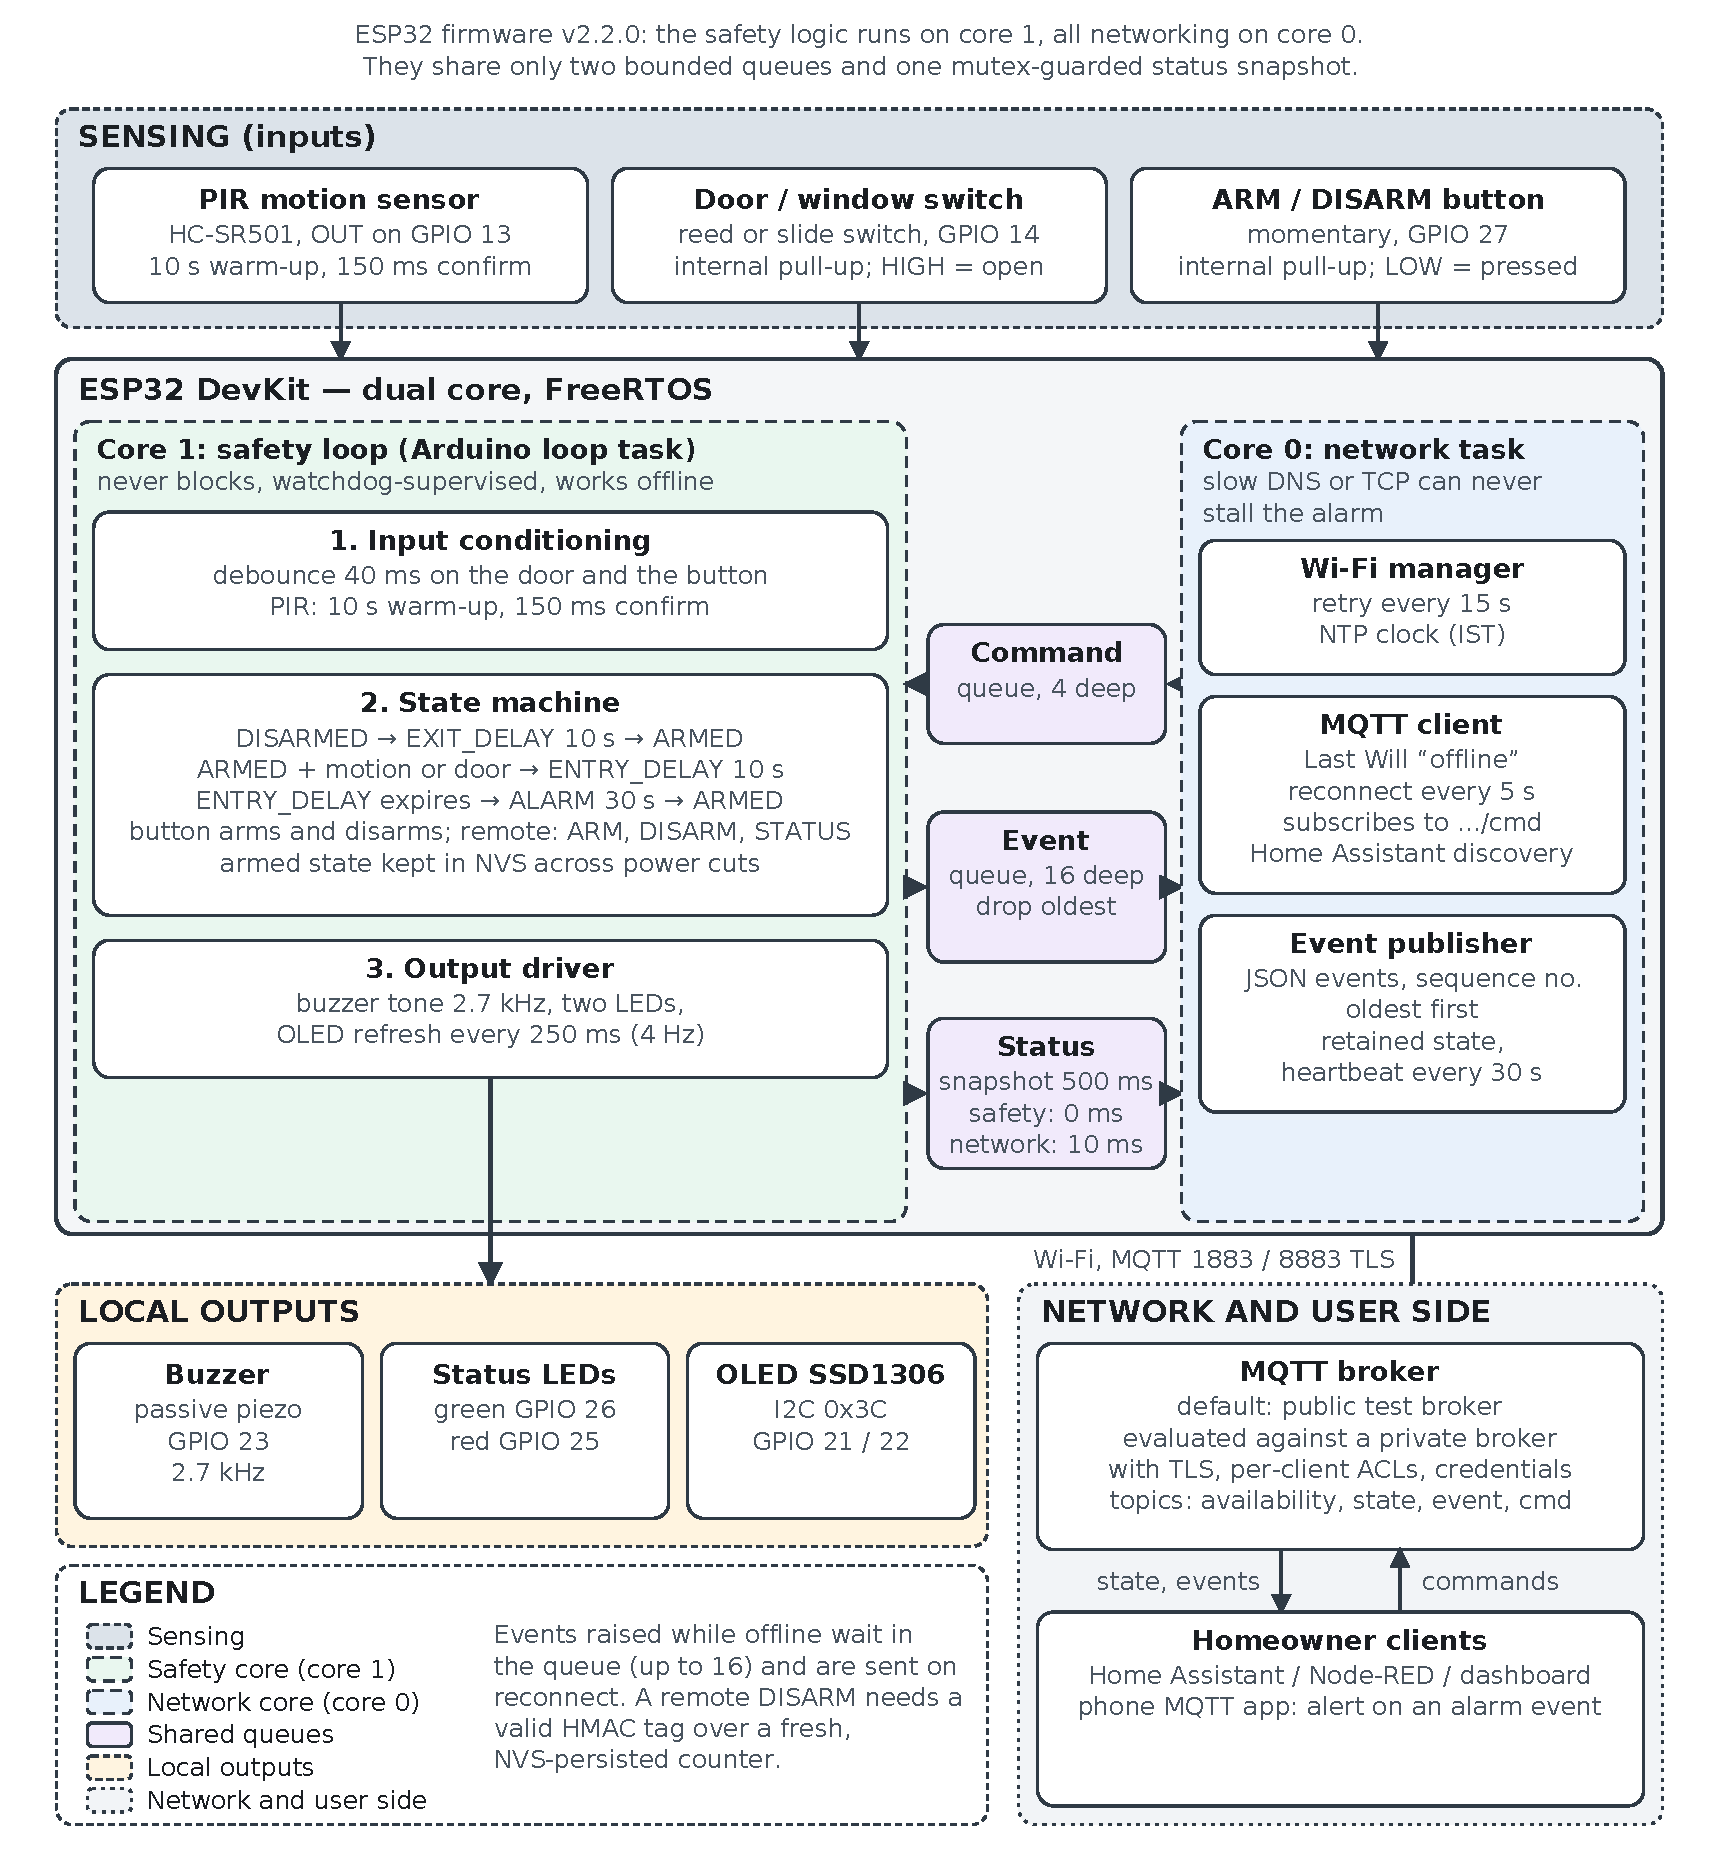
\includegraphics[width=0.92\textwidth]{architecture.pdf}
\caption{System architecture. The safety domain on core~1 owns the state machine, sensing and
actuation; the network domain on core~0 owns Wi-Fi, MQTT and command authentication. The two
communicate only through two bounded queues and a status snapshot guarded by a zero-timeout
mutex.}
\label{fig:arch}
\end{figure}

Three mechanisms enforce the separation, and each addresses a distinct failure mode.

\emph{Core pinning} prevents the network task from occupying the safety core's execution slot.
The network task is created with an explicit core affinity; the safety loop runs as the default
application task on the other core.

\emph{Bounded queues} prevent either side from exhausting the other's memory or blocking it. The
event queue (safety to network) holds sixteen entries and the command queue (network to safety)
holds four. On overflow the oldest event is discarded \emph{and counted}, so loss is observable
rather than silent; the published device state carries the drop count.

\emph{A zero-timeout status snapshot} prevents priority inversion from reaching the safety side.
The asymmetry here is the mechanism and is easy to overlook: the safety loop acquires the status
mutex with a timeout of zero and simply skips the update if the network task holds it, while the
network task may wait up to 10\,ms. Contention can therefore delay the network side and never the
safety side.

\subsection{Command authentication}

Remote commands carry an authentication tag and a counter. With shared key $K$ and message
$m = \texttt{VERB}\,\|\,\text{``:''}\,\|\,c$ for counter $c$, the transmitted tag is
\begin{equation}
\tau = \mathrm{trunc}_{16}\!\left(\mathrm{HMAC\text{-}SHA256}(K, m)\right),
\label{eq:tag}
\end{equation}
where $\mathrm{HMAC}$ follows RFC~2104 and truncation to 16 octets is permitted by its
Section~5, giving a forgery probability of $2^{-128}$ per attempt. A command is accepted iff
\begin{equation}
\mathrm{ct\_eq}\!\left(\tau, \tau'\right) \;\wedge\; c > c_{\text{stored}},
\label{eq:accept}
\end{equation}
where $\tau'$ is the recomputed tag, $\mathrm{ct\_eq}$ is a constant-time comparison that
accumulates differences rather than returning early, and $c_{\text{stored}}$ is the counter held
in non-volatile storage. Both conjuncts are necessary and they defend different things: the
first defeats forgery, the second defeats replay. Section~\ref{sec:results} shows empirically
that a design with only the first is broken by capture-and-replay.

Two placement decisions matter more than the construction, which is standard.

The expensive verification runs on $C_{n}$, before the command queue. A flood of forged commands
is therefore rejected entirely within the network domain and consumes no safety-core time; only
a verdict and an enumerated verb cross the boundary. Figure~\ref{fig:cmdflow} shows the path.

The counter is committed to non-volatile storage \emph{before} the command is acted upon. Were
the order reversed, an interruption between action and commit would leave the command replayable.
In the chosen order the worst case is that a counter value is consumed without the command
executing, which fails safe: a legitimate sender increments and retries, while an adversary gains
nothing.

\begin{figure}[t]
\centering
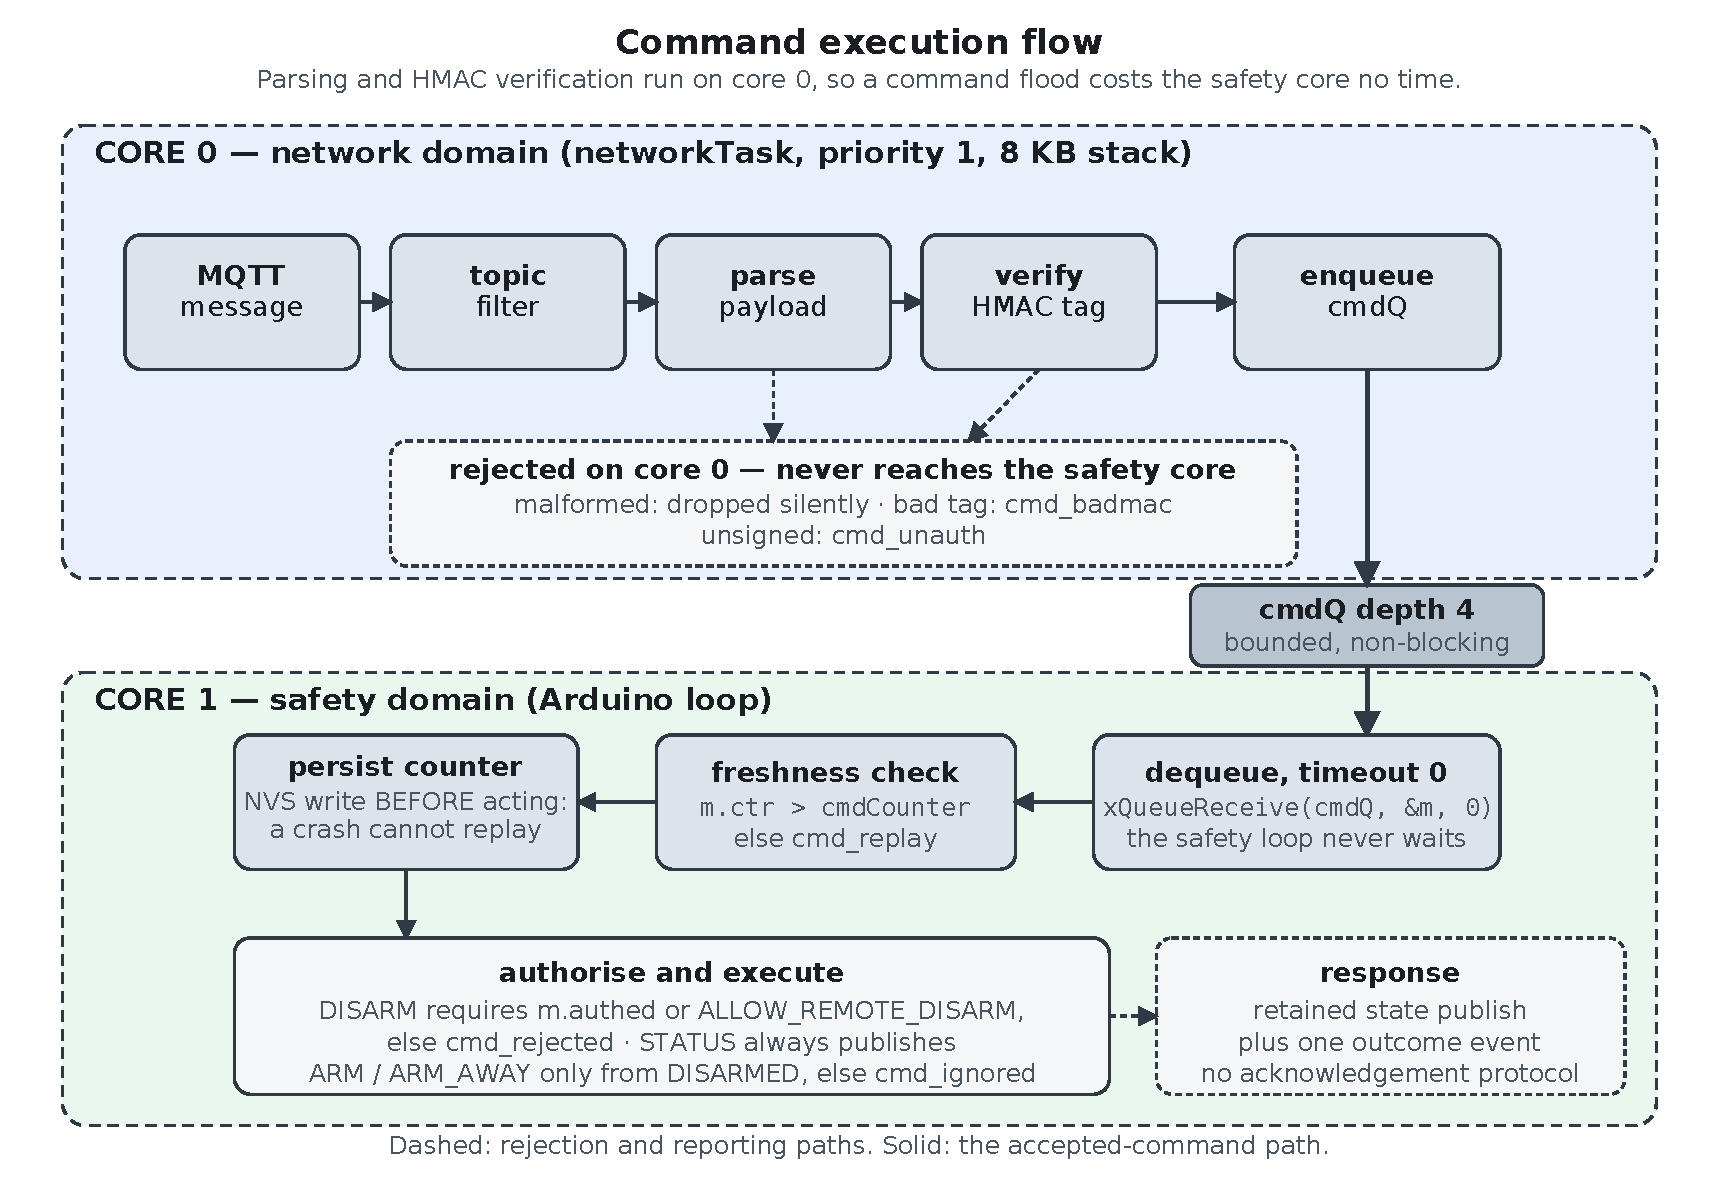
\includegraphics[width=0.92\textwidth]{command_flow.pdf}
\caption{Command execution across the two cores. Parsing and tag verification complete on core~0,
so a command flood costs the safety core no time; the replay counter is committed to
non-volatile storage before the command is acted upon.}
\label{fig:cmdflow}
\end{figure}

\subsection{Supporting mechanisms}

A passive detector counts 802.11 deauthentication and disassociation frames in a sliding window
and raises an event when the count reaches a threshold, subject to a cooldown that bounds the
report rate. Writing $N(t)$ for the number of such frames in $(t-W,\,t]$, the detector reports at
$t$ iff
\begin{equation}
N(t) \ge T \;\wedge\; t - t_{\text{last}} > C .
\label{eq:deauth}
\end{equation}
The detector never transmits. The cooldown is not cosmetic: without it the detector could itself
flood the bounded event queue, converting a radio attack into a denial of service against the
notification path. Parameters $T$ and $W$ were chosen by the sweep in
Section~\ref{sec:results}, which overturned our initial choice.

When the broker is unreachable the device can send a signed, counter-protected alert to a second
device over ESP-NOW, which operates without an access point. Optional sensor fusion requires
agreement between a passive infrared sensor and a millimetre-wave radar within a window $W_{f}$,
reducing single-sensor false alarms. Armed state and the command counter persist in non-volatile
storage, so a power interruption while armed does not silently disarm the system.

\section{Formal Verification}\label{sec:formal}

We specify two models in TLA+~\cite{lamport2002} and check them exhaustively with TLC.

\subsection{State machine and command path}

The first specification models the five alarm states, the transitions between them and the
command rules. Over all 25 reachable states at the configured counter bound, TLC verifies that no
unauthenticated remote command disarms the system, that the replay counter never decreases, that
the siren is never active while disarmed, and that the entry delay and the alarm always resolve
rather than deadlocking.

\subsection{The isolation argument}

The second specification is the one that carries the paper's design claim. It models both tasks,
with the network task made maximally adversarial: it may become busy, stall for an unbounded
time, fail to publish, crash and restart, and it is granted \emph{no fairness}. Weak fairness is
asserted for the safety step alone:
\begin{equation}
\mathit{Spec} \;\triangleq\; \mathit{Init} \wedge \Box[\mathit{Next}]_{\mathit{vars}} \wedge
\mathrm{WF}_{\mathit{vars}}(\mathit{SafetyStep}).
\label{eq:spec}
\end{equation}
Table~\ref{tab:properties} lists the verified properties. TLC explored 2{,}686 states, 660 of
them distinct, to a graph depth of 26, with no violation.

\begin{table}[t]
\centering\small
\caption{Properties verified by TLC. Both specifications were additionally mutation-tested.}
\label{tab:properties}
\begin{tabular}{@{}llp{0.48\textwidth}@{}}
\toprule
Property & Type & Statement \\
\midrule
\textsc{NoUnauthRemoteDisarm} & invariant & No unauthenticated remote command causes a transition to the disarmed state \\
\textsc{CounterMonotonic}     & property  & The replay counter never decreases \\
\textsc{NoAlarmWhenDisarmed}  & invariant & The siren is never active in the disarmed state \\
\textsc{SafetyCanAlwaysStep}  & invariant & The safety step is enabled whenever work remains \\
\textsc{NoNetworkWrite}       & invariant & The network task never writes alarm state \\
\textsc{QueueBounded}         & invariant & The event queue never exceeds its capacity \\
\textsc{NoSilentLoss}         & invariant & produced $=$ delivered $+$ queued $+$ dropped \\
\textsc{EntryLeadsToResolve}  & liveness  & An entry delay always ends in alarm or disarm \\
\textsc{SafetyProgress}       & liveness  & The safety function makes progress \\
\bottomrule
\end{tabular}
\end{table}

\subsection{Mutation testing}

A model checker reports no violation for a vacuous specification as readily as for a sound one.
We therefore injected defects corresponding to each property and confirmed that TLC reports the
expected violation: permitting an unauthenticated disarm violates
\textsc{NoUnauthRemoteDisarm}, and allowing the network task to write alarm state violates
\textsc{NoNetworkWrite}. The properties therefore have force.

\subsection{What the models do not cover}

The abstraction boundary deserves explicit statement, because it is exactly where the research
question lives. The network task is modelled as a set of discrete actions, not as a source of
\emph{timing interference}. TLC establishes that within this abstraction no control- or data-flow
dependency can block the safety step. It says nothing about contention for shared silicon, which
is a property of the implementation rather than the model. Model checking here bounds the logical
design space; it does not substitute for measurement.

\section{Implementation}\label{sec:impl}

The firmware comprises approximately 1{,}100 lines of C++ for the main application, together
with four self-contained headers. These provide a portable SHA-256 and HMAC-SHA256
implementation, checked against the published RFC~4231 test vectors; the deauthentication
detector; the signed out-of-band alert message; and the sensor-fusion logic. The three latter headers contain pure logic with no platform
dependency, which allows them to be tested on a host without hardware.

\subsection{Verification infrastructure}

The unmodified firmware compiles against host models of Arduino, FreeRTOS, Wi-Fi, MQTT,
non-volatile storage and the display. The firmware source is not altered for testing, which is
what makes the simulation results meaningful. The suite runs nineteen scenarios at three clock
start values across two vendor framework versions, plus build-configuration and header-synchrony
checks, for 120 checks in total.

The three clock start values include one immediately below the 32-bit wrap of the millisecond
counter. All elapsed-time comparisons are written in the wrap-safe form
$(\texttt{uint32\_t})(\mathit{now} - \mathit{since}) \ge \mathit{interval}$ rather than
$\mathit{now} \ge \mathit{since} + \mathit{interval}$, which fails at the boundary. This is not a
theoretical concern: a defect of exactly this class, under which the siren could remain active
after approximately 25 days of uptime, was found by this method during development.

\subsection{Resource cost}

Table~\ref{tab:build} gives flash and RAM consumption as reported by the compiler for both
framework versions. The security features added in the hardened configuration cost
approximately 3\,kB of flash and 170\,bytes of RAM. We emphasise that this is a static measure:
no CPU-time or energy cost has been measured, and both remain open.

\begin{table}[t]
\centering\small
\caption{Build cost, as reported by the compiler in continuous integration. Static sizes only;
no run-time or energy cost has been measured.}
\label{tab:build}
\begin{tabular}{@{}lrrrr@{}}
\toprule
Framework version & Flash (B) & of budget & RAM (B) & of budget \\
\midrule
arduino-esp32 2.0.17 & 793{,}433 & 60.5\% & 46{,}372 & 14.2\% \\
arduino-esp32 3.3.12 & 968{,}221 & 73.9\% & 49{,}876 & 15.2\% \\
\bottomrule
\end{tabular}
\end{table}

\section{Experimental Methodology}\label{sec:method}

\subsection{Evidence categories}

Results in this paper fall into three categories and we label each one, because they are not
interchangeable. \emph{Formal verification results} come from exhaustive model checking.
\emph{Simulation results} come from the unmodified firmware driven by a seeded harness on a host.
\emph{Analytical results} follow from the construction, such as the $2^{-128}$ forgery
probability. No result in this paper is a physical hardware measurement; the single exception
is the build cost of Table~\ref{tab:build}, which a real compiler measured but which describes
the binary rather than the running device.

\subsection{Hypotheses}

\begin{description}[leftmargin=1.6em,itemsep=0.2em]
\item[H1 (logical isolation).] No execution of the system exists in which network activity
blocks, delays or corrupts the safety path, and no forged, stale or malformed command is
accepted. \emph{Testable by model checking and simulation.}
\item[H2 (timing isolation).] $F_{\Lambda} \stackrel{d}{=} F_{0}$ for radio-layer load $\Lambda$
across the operating range. \emph{Requires hardware; not tested here.}
\end{description}

Given~\cite{behnke2020}, we do not expect H2 to hold exactly. The informative question is the
magnitude of any shift relative to the deadline margin, and whether queue discipline bounds it.

\subsection{Determinism and reproduction}

Nothing in the evaluation is collected as a dataset. Inputs are generated deterministically from
fixed seeds, which is stronger for this purpose than distributing a file: an independent
researcher regenerates the identical inputs by running the scripts. Each trial of the adversarial
campaign and the ablation executes in a forked child process, because the firmware's globals are
file-scope and would otherwise leak between trials. This was not a stylistic choice: before it
was introduced, state leakage produced a spurious invariation violation at zero attack rate.

The campaign and fuzzing pipeline has been verified to regenerate its summary files
byte-identically from the committed seeds.

\subsection{Metrics}

\begin{table}[t]
\centering\small
\caption{Evaluation metrics and their definitions.}
\label{tab:metrics}
\begin{tabular}{@{}lp{0.62\textwidth}@{}}
\toprule
Metric & Definition \\
\midrule
Safety latency & Simulated milliseconds from confirmed sensor assertion to entry-delay entry \\
Command availability & Trials in which a legitimate command issued during the flood took effect \\
Integrity failure & Trials in which an adversary's message caused a state change \\
Replay defeat & Trials in which the adversary obtained an accepted command using only captured or forged material \\
Invariant violation & Trials violating any safety invariant \\
Accepted fuzz input & Inputs changing state or advancing the counter without a valid tag \\
False-positive rate & Benign runs in which the detector reported at least once \\
Detection latency & Simulated milliseconds from attack onset to first detector report \\
\bottomrule
\end{tabular}
\end{table}

\subsection{Experimental configurations}

The adversarial campaign runs 3{,}000 trials per build across six attack rates from 0 to
20{,}000~messages/s. The adversary injects forged tags signed with a key it does not hold,
replays of messages captured on the wire, bare verbs carrying no credential, and random bytes.
The ablation runs 300 trials per design over the same rates with identical seeds. The fuzzer
runs 3{,}000{,}000 iterations over six input classes under AddressSanitizer and
UndefinedBehaviorSanitizer. The sensitivity sweep runs 2{,}000 benign trials of ten simulated
minutes per grid cell.

\section{Results}\label{sec:results}

\subsection{Adversarial campaign}

Across 6{,}000 trials no adversary disarmed the device and no safety invariant was violated.
Without command authentication the adversary changed the system state in all 2{,}500 flooded
trials; with authentication, in none. The availability result is the more informative one: with
authentication a legitimate command took effect in all 3{,}000 trials regardless of attack rate,
while in the baseline flooding starved it in every flooded trial.

We report no hypothesis test on these data. Because the harness advances a logical clock there
is no contention, the safety latency is a deterministic 151\,ms in every trial---the sensor
confirmation window plus loop period---and its variance is identically zero. Any test on two
constant-valued samples is trivially satisfied and carries no information. We pre-register the
analysis for the hardware measurements instead: a two-sided Mann--Whitney $U$ test with tie
correction, chosen because latency distributions on a real-time operating system are not normal,
with the implementation committed in advance.

\subsection{Command-path ablation}

To avoid resting on a baseline that is defeated by construction, we ran the same adversary
against four designs: no command defence, a token-bucket rate limiter admitting five commands per
second, a static shared token carried in the payload, and the signed-counter path. The rate
limiter and the token are modelled as edge filters, which is where a developer would place them
in practice. Table~\ref{tab:ablation} reports the outcome.

\begin{table}[t]
\centering\small
\caption{Command-path ablation. 300 trials per design, identical adversary and seeds.
``Survives flood'' counts flooded trials in which a legitimate command took effect; ``defeated by
replay'' counts trials in which the adversary obtained an accepted command using only captured or
forged material.}
\label{tab:ablation}
\begin{tabular}{@{}lccc@{}}
\toprule
Design & Survives flood & Defeated by replay & Alarm fired \\
\midrule
No command defence            & 0/250            & 250/300          & 300/300 \\
Rate limit, 5 commands/s      & 0/250            & 246/300          & 300/300 \\
Static shared token           & 250/250          & 250/300          & 300/300 \\
\textbf{HMAC-SHA256 + counter}& \textbf{250/250} & \textbf{0/300}   & \textbf{300/300} \\
\bottomrule
\end{tabular}
\end{table}

The result separates two properties that are easily conflated. A rate limiter cannot distinguish
a legitimate command from a flood, so it discards both and sacrifices availability while leaving
integrity entirely untouched. A static shared token \emph{does} restore availability, because the
edge filters the flood cheaply---but it travels in plaintext, so a single captured command
defeats it. Only the monotonic counter prevents replay; a message authentication code alone would
behave as the token row does. The practical implication is that a designer evaluating a
command-path defence against availability alone will accept a design that is trivially broken on
integrity.

The alarm fired in every trial of every design. This is the isolation property behaving as
intended: the safety function does not depend on the command path, so no command-path design
choice affects whether the siren sounds.

\subsection{Detector parameter sensitivity}

The detector's threshold and window had a stated rationale but no measurement. Sweeping them against a Poisson model of benign management-frame arrivals showed that our initial
threshold of eight was wrong. Access points emit deauthentication and disassociation frames in
normal operation during roaming, idle timeout, load balancing and reboot; at 60 frames per minute,
representing a busy multi-access-point environment, a threshold of eight fired spuriously in
79.9\% of ten-minute runs. Table~\ref{tab:sensitivity} gives the trade-off surface.

\begin{table}[t]
\centering\small
\caption{Detector sensitivity. False-positive rate is measured at 60 benign frames per minute;
detection latency is the median at the stated attack rate. The deployed configuration is shown
in bold.}
\label{tab:sensitivity}
\begin{tabular}{@{}rrrrrr@{}}
\toprule
Threshold & Window (ms) & FP rate & Detect, 20 f/s & Detect, 5 f/s & Missed, 5 f/s \\
\midrule
5  & 2000 & 1.0000 & 234\,ms & 948\,ms  & 0/500 \\
8  & 1000 & 0.0355 & 405\,ms & 2326\,ms & 0/500 \\
8  & 2000 & 0.7985 & 383\,ms & 1520\,ms & 0/500 \\
\textbf{12} & \textbf{2000} & \textbf{0.0025} & \textbf{597\,ms} & \textbf{2673\,ms} & \textbf{0/500} \\
12 & 5000 & 0.9450 & 577\,ms & 2348\,ms & 0/500 \\
20 & 2000 & 0.0000 & 1004\,ms & 26137\,ms & 279/500 \\
20 & 5000 & 0.0005 & 958\,ms & 3852\,ms & 0/500 \\
\bottomrule
\end{tabular}
\end{table}

We revised the firmware default to twelve, which reduces the false-positive rate to 0.25\% while
still detecting every attack rate swept with no misses, at a cost of approximately 214\,ms of
additional detection latency at 20 frames per second. A detector that reports frequently on a
healthy network trains its owner to ignore it, and on this device each report consumes an
event-queue slot; the additional latency is a reasonable price.

We are explicit that the benign arrival model is an \emph{assumption}, not a measurement. No
capture of real management-frame traffic was available to us. These results therefore
characterise the detector's logic against a stated model and are not a false-positive rate for
any real network. Obtaining one requires a passive capture on a production network and is
future work.

\subsection{Fuzzing}

The command parser is the one input a network peer fully controls. Across 3{,}000{,}000
iterations under AddressSanitizer and UndefinedBehaviorSanitizer the fuzzer found no memory
error, no undefined behaviour, and no input that changed state or advanced the counter. We read
this as evidence of memory safety and parser robustness rather than of authentication soundness:
against a 128-bit tag, zero forgeries is the expected outcome and is not independent evidence.

One episode is worth recording as a methodological caution. An early run reported an accepted
input. Investigation showed the mutation had flipped the case of a hexadecimal digit, which
decodes to identical tag bytes, so the input was the genuine command and acceptance was correct
behaviour. The corpus now signs its mutation seed with a deliberately incorrect key so that no
mutation can produce a valid command by accident. Had this not been chased down it would have
become a false claim.

\section{The Open Experiment: Physical Timing Invariance}\label{sec:hw}

The results above establish H1. They cannot establish H2, because the simulated clock does not
model contention for the bus, the cache or the interrupt controller, and that contention is
precisely the phenomenon in question. We therefore specify the measurement rather than
approximate it.

\subsection{Apparatus}

Figure~\ref{fig:setup} shows the arrangement. The device under test runs the unmodified
firmware. A second, independent microcontroller acts as the measuring instrument: it drives the
sensor line, timestamps that edge with its own hardware timer, and timestamps the rising edge of
the siren line. The measuring clock is therefore never the clock under load, which is essential:
a device cannot credibly measure its own latency while that latency is the quantity being
perturbed.

\begin{figure}[t]
\centering
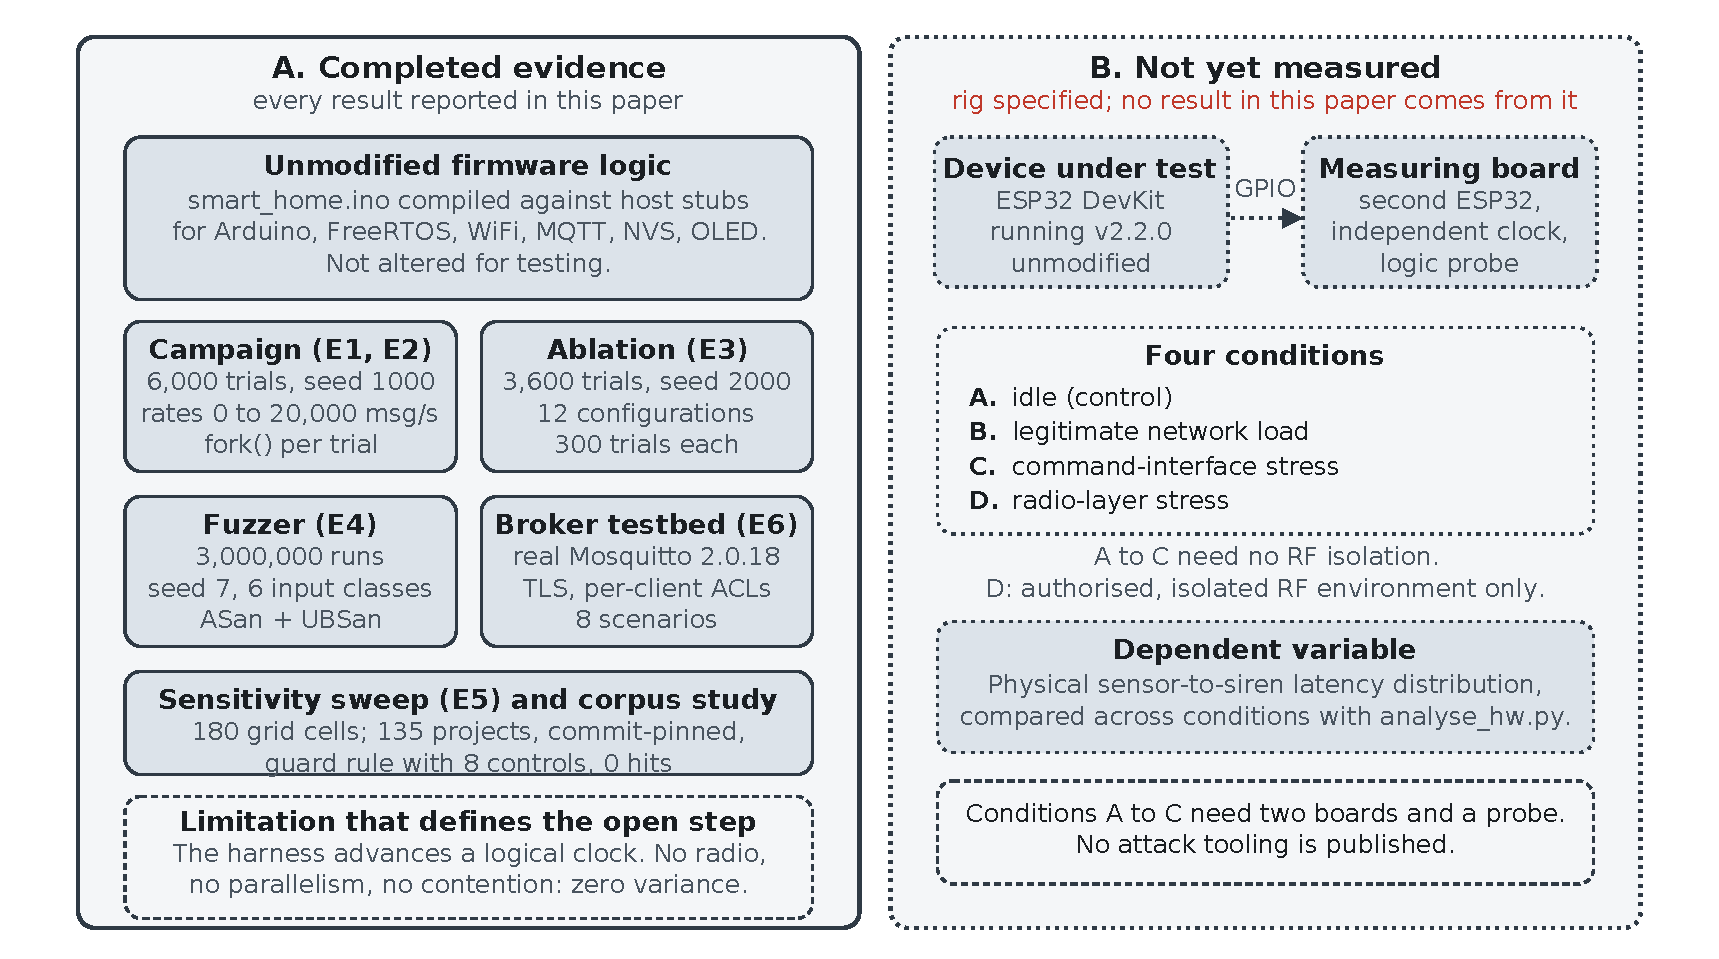
\includegraphics[width=0.92\textwidth]{experimental_setup.pdf}
\caption{Experimental setup. (A) The simulation harness used for all results reported in this
paper. (B) The hardware rig, specified and built but not yet run, in which a second
microcontroller serves as an independent measuring instrument across four load conditions.}
\label{fig:setup}
\end{figure}

\subsection{Conditions}

Four conditions, each compared against the unloaded control:

\begin{description}[leftmargin=1.6em,itemsep=0.15em]
\item[A. Idle.] No network activity. Establishes $F_{0}$ and the instrument's own noise floor.
\item[B. Legitimate load.] Normal MQTT traffic with the broker reachable.
\item[C. Command-interface stress.] High-rate publication on the command topic.
\item[D. Radio-layer stress.] Deauthentication and disassociation frames at the MAC layer.
\end{description}

Conditions A through C require only the two boards and a probe. Condition D requires an
authorised isolated or shielded radio environment and institutional permission, and is the
condition that distinguishes this work from prior IP-layer measurements.

\subsection{Analysis plan, pre-registered}

Each loaded condition is compared against condition~A using a two-sided Mann--Whitney $U$ test
with tie correction. For samples of size $n_1$ and $n_2$ with rank sum $R_1$,
\begin{align}
U_1 &= R_1 - \frac{n_1(n_1+1)}{2}, \qquad U = \min(U_1,\, n_1 n_2 - U_1), \label{eq:u}\\
\sigma_U^2 &= \frac{n_1 n_2}{12}\left[(n+1) - \frac{\sum_i (t_i^3 - t_i)}{n(n-1)}\right],
\qquad n = n_1 + n_2, \label{eq:sigma}
\end{align}
with $z = (U - n_1 n_2 / 2)/\sigma_U$ and a two-sided $p$-value from the normal approximation.
The test is non-parametric because latency distributions on a real-time operating system are not
normal. The bracketed term in~\eqref{eq:sigma} is the tie correction, which matters here because
quantised timer readings produce many ties. The implementation is committed in advance of any
measurement, and we will report effect size and the full distribution rather than a $p$-value
alone.

\subsection{Ethics}

The radio-layer condition is to be performed only on equipment owned by the experimenter, in an
isolated or shielded environment, with institutional permission obtained beforehand. No
third-party network or device is targeted. Neither this paper nor its public repository contains
any attack-generation procedure or tooling. We note that deauthentication tooling for this chip
family is already published~\cite{deauther2026,espwn2023}; we cite that work as evidence the
threat is realistic while declining to add to it.

\section{Discussion}\label{sec:discussion}

\subsection{What the evidence supports}

The formal and simulation results together establish that the design contains no path by which
network activity reaches the safety function logically. The TLA+ isolation model is the stronger
of the two, because granting the network task no fairness means the property holds under every
possible interleaving rather than the ones a harness happens to generate. The campaign and
fuzzing results confirm that the implementation matches the specification.

The ablation is the result we consider most likely to be useful to other designers, because it is
the least predictable. It is tempting to evaluate a command-path defence by asking whether
legitimate commands survive an attack. Both the static token and the signed-counter design pass
that test identically, and a designer stopping there would conclude they are equivalent. They are
not: one is defeated by a passive eavesdropper, and the measurement that distinguishes them is
capture-and-replay rather than throughput.

\subsection{Why the design behaves as observed}

The availability result follows from where verification happens rather than from cryptography.
Because the tag is checked on the network core before the bounded command queue, a flood of
invalid commands is discarded without ever occupying a queue slot. The queue therefore retains
capacity for the one valid command, and admission is decided by validity rather than arrival
order. A rate limiter inverts this: it decides by arrival order, which an attacker controls.

\subsection{Relationship to prior measurement}

Our work complements rather than contradicts~\cite{behnke2020}. They established that on-chip
network activity reaches a critical task on this hardware even with cross-core separation; we
accept that result and address the question it leaves open, namely whether the mitigations
available on stock hardware are adequate, under the load class that actually threatens a wireless
alarm. Their proposed mitigations require either hardware that does not
exist~\cite{behnke2022} or a platform an order of magnitude larger~\cite{behnke2023}. If our
pending measurement shows that pinning with queue discipline holds the deadline under radio-layer
load, that is a useful positive result for a very large installed base. If it shows the opposite,
that is a more important result still, because it would indicate that the standard advice given
to developers of such devices is insufficient and that the installed base is exposed.

\section{Threats to Validity}\label{sec:threats}

\paragraph{Construct validity.} This is the most serious threat. The dependent variable in
simulation is a logical latency measured on a clock the harness itself advances. We call it
safety latency, but it is not the physical quantity of interest, and the divergence between the
construct and the measure is the reason Section~\ref{sec:hw} exists.

\paragraph{Internal validity.} Largely controlled. Seeds are fixed, the pipeline regenerates
byte-identically, and continuous integration re-runs a reduced version on every commit.
Per-trial process isolation was introduced specifically because global state leakage had produced
a spurious violation. Two further harness defects were found during the ablation and are
documented: the adversary could act during the experimenter's own control actions, and could
leave the system mid-transition so that the intrusion phase was skipped, which made the weaker
designs appear to fail in a way they had not. The residual threat is that the host models and
the firmware share an author, so a common misconception would be invisible to both.

\paragraph{External validity.} Limited, and we scope our claims accordingly. All results concern
one chip, two framework versions, one application and no deployment. We do not generalise to
single-chip Wi-Fi SoCs as a class. The single-core variants of the same family are arguably the
more interesting case, since they cannot pin at all.

\paragraph{Conclusion validity.} We report no statistical conclusion from the simulation,
precisely because the zero-variance data cannot support one. The formal conclusions are sound
within their abstraction, and that abstraction excludes timing. The security conclusions of the
campaign follow deductively from the construction and are therefore valid but uninformative;
the ablation was added because of this.

\paragraph{Bias.} There is no blinding, and the analysis author is the implementation author. For
the hardware campaign this matters more than it does in simulation, because expectancy effects
can influence setup and outlier handling. The measurement protocol and the analysis script are
committed before any data is collected, which is a pre-registration in substance.

\section{Limitations and Future Work}\label{sec:limitations}

The principal limitation is stated plainly: no physical measurement has been performed, and the
timing-invariance claim is consequently untested. No latency figure appears in this paper that we
have not measured, and none is estimated.

Beyond this: the benign arrival model underlying the sensitivity analysis is synthetic; the
per-command CPU cost of tag verification and the energy cost of both the security features and
promiscuous-mode monitoring are unmeasured; the ablation lacks an arm representing transport
security with broker credentials; no ablation isolates the contribution of each of the four
security mechanisms individually; flash encryption, secure boot and signed over-the-air update
are not implemented; and the false-alarm rate of the sensor-fusion modes has not been
characterised against real sensors.

The ordered priorities for future work are therefore: conditions A through C of the hardware
protocol, which need only two boards and a probe; condition D, subject to approval; a passive
capture to replace the synthetic arrival model; and replication on a single-core variant of the
same family.

\section{Conclusion}\label{sec:conclusion}

We treated a consumer intrusion alarm as a safety-critical system and asked whether the one
isolation mitigation available on its hardware---core pinning, combined with bounded queue
discipline---is adequate when the attacked resource is the chip's own radio. Prior measurement
establishes that network activity reaches a critical task on this hardware despite cross-core
separation; what it does not establish is whether the available mitigation suffices, and it has
not examined radio-layer load, an adversarial model, or any formal treatment.

We answer the logical half of the question with exhaustive model checking under a network task
granted no fairness, with 7{,}200 seeded adversarial trials and with three million
sanitizer-backed fuzzing iterations. We show through ablation that availability and integrity are
separable properties and that a plausible defence can satisfy the first while failing the second
completely. We show through sensitivity analysis that our own initial detector threshold was
wrong by a wide margin, and we corrected it. We specify in full the one measurement that settles
the timing half, and we report no number for it, because we have not made it.

All claims are scoped to the platform tested: the dual-core Xtensa ESP32 under arduino-esp32
2.0.17 and 3.3.12. The artifact is public so that the results can be reproduced and the open
measurement completed, by us or by others.

\section*{Declarations}

\noindent\textbf{Funding.} This research received no external funding.

\noindent\textbf{Conflicts of interest.} The author declares no conflict of interest.

\noindent\textbf{Author contributions.} MD Humayun: conceptualisation, methodology, software,
formal analysis, investigation, data curation, writing (original draft, review and editing),
visualisation.

\noindent\textbf{Data availability.} All data reported here are generated deterministically from
fixed seeds by scripts in the public repository. Aggregate results and the raw per-trial records
for the ablation and sensitivity experiments are committed; the campaign's per-trial records
regenerate identically by running the provided script. No third-party or human-subject data were
used.

\noindent\textbf{Code availability.} Firmware, formal specifications, experiment harnesses,
analysis scripts and figure sources are publicly available under the MIT licence. Continuous
integration re-runs the formal verification and a reduced adversarial campaign on every commit.

\noindent\textbf{Ethics.} No human or animal subjects were involved, and no third-party network,
device or system was attacked or tested. The repository publishes no attack-generation procedure
or tooling.

\section*{Acknowledgements}

\noindent\textbf{Use of AI-assisted tools.} An AI assistant was used for drafting assistance,
documentation, code review and literature discovery. All research claims, experimental designs,
results and conclusions are the author's own. Every result reported here was produced by the
committed scripts and verified by the author, and every reference was checked against its
publisher or preprint record.

\begin{thebibliography}{99}
\small

\bibitem{behnke2020} I.~Behnke, L.~Pirl, L.~Thamsen, R.~Danicki, A.~Polze, and O.~Kao,
``Interrupting real-time IoT tasks: How bad can it be to connect your critical embedded system to
the Internet?,'' in \emph{Proc.\ IEEE 39th Int.\ Performance Computing and Communications Conf.\
(IPCCC)}, 2020.

\bibitem{behnke2022} I.~Behnke, P.~Wiesner, R.~Danicki, and L.~Thamsen, ``A priority-aware
multiqueue NIC design for real-time IoT devices,'' in \emph{Proc.\ 37th ACM/SIGAPP Symp.\ on
Applied Computing (SAC)}, 2022. doi:10.1145/3477314.3507165.

\bibitem{behnke2023} I.~Behnke, C.~Blumschein, R.~Danicki, P.~Wiesner, L.~Thamsen, and O.~Kao,
``Towards a real-time IoT: Approaches for incoming packet processing in cyber-physical systems,''
\emph{Journal of Systems Architecture}, vol.~140, art.~102891, 2023.
doi:10.1016/j.sysarc.2023.102891.

\bibitem{fischer2020} F.~Fischer \emph{et al.}, ``Analysis of industrial device architectures for
real-time operations under denial of service attacks,'' arXiv:2007.08885, 2020.

\bibitem{timingiso2025} L.~Meszl\'enyi, J.~Kahle, D.~P\"ullen, S.~Kowalewski, S.~Katzenbeisser,
and A.~Kampmann, ``Towards timing isolation for mixed-criticality communication in
software-defined vehicles,'' arXiv:2508.13652, 2025.

\bibitem{mcti2024} D.~Hoornaert, G.~Ghaemi, A.~Bastoni, R.~Mancuso, M.~Caccamo, and G.~Corradi,
``Mcti: Mixed-criticality task-based isolation,'' \emph{Real-Time Systems}, vol.~60, no.~2,
pp.~328--365, 2024. doi:10.1007/s11241-024-09425-5.

\bibitem{mcreview2026} A.~Burns and R.~I.~Davis, ``Mixed criticality systems: A review,'' 14th
edn., Dept.\ of Computer Science, University of York, Feb.\ 2026.

\bibitem{deauther2026} S.~Kremser and K.~Graffi, ``Evaluating the ESP32-S3 for Wi-Fi penetration
testing through the development of Deauther32 and HackHeld32,'' \emph{Sensors}, vol.~26, no.~11,
art.~3287, 2026. doi:10.3390/s26113287.

\bibitem{espwn2023} R.~Cayre, D.~Cauquil, and A.~Francillon, ``ESPwn32: Hacking with ESP32
system-on-chips,'' in \emph{Proc.\ 17th IEEE Workshop on Offensive Technologies (WOOT)}, 2023.

\bibitem{carbajal2026} A.~Carbajal and A.~Jodeiri Akbarfam, ``A software-defined testbed for
quantifying deauthentication resilience in modern Wi-Fi networks,'' arXiv:2602.23513, 2026.

\bibitem{esp32c3re2025} I.~Mudraje, K.~Vogelgesang, J.~Devreker, L.~Gerhorst, P.~Raffeck,
P.~W\"agemann, and T.~Herfet, ``Reverse engineering the ESP32-C3 Wi-Fi drivers for static
worst-case analysis of intermittently-powered systems,'' arXiv:2501.17684, 2025.
doi:10.1145/3722572.3727926.

\bibitem{mqtttls2026} M.~A.~Azhar, M.~Azwar, and O.~Asroni, ``Performance and security analysis
of MQTT over TLS on ESP32-based IoT systems,'' \emph{J.\ Applied Informatics and Computing},
2026.

\bibitem{ondevice2026} V.~Ieropoulos \emph{et al.}, ``Empowering IoT security: On-device
intrusion detection in resource constrained devices,'' arXiv:2605.13159, 2026.

\bibitem{krichen2023} M.~Krichen, ``A survey on formal verification and validation techniques for
Internet of Things,'' \emph{Applied Sciences}, vol.~13, no.~14, art.~8122, 2023.
doi:10.3390/app13148122.

\bibitem{lamport2002} L.~Lamport, \emph{Specifying Systems: The TLA+ Language and Tools for
Hardware and Software Engineers}. Addison-Wesley, 2002.

\bibitem{fuzzsurvey2022} J.~Yun \emph{et al.}, ``Fuzzing of embedded systems: A survey,''
\emph{ACM Computing Surveys}, 2022. doi:10.1145/3538644.

\bibitem{pemu2025} M.~Bley, T.~Scharnowski, S.~W\"orner, M.~Schloegel, and T.~Holz,
``Protocol-aware firmware rehosting for effective fuzzing of embedded network stacks,'' ACM,
2025. doi:10.1145/3719027.3765125.

\bibitem{sysfuss2026} D.~Tharindu, A.~Jayasena, and P.~Mishra, ``SysFuSS: System-level firmware
fuzzing with selective symbolic execution,'' arXiv:2602.02243, 2026.

\end{thebibliography}

\end{document}
